\documentclass[tikz,border=3.14mm]{standalone}
\usepackage{pgfplots}
\pgfplotsset{compat=1.18}

% Define colors
\definecolor{arr2flatcolour}{RGB}{31, 119, 180}    % Blue
\definecolor{minnesotacolour}{RGB}{255, 127, 14}    % Yellow
\definecolor{gaussiancolour}{RGB}{44, 160, 44}     % Green
\definecolor{rhscolour}{RGB}{148, 103, 189}        % Purple
\definecolor{arr2minncolour}{RGB}{214, 39, 40}     % Red
\definecolor{arr2bumpcolour}{RGB}{140, 168, 214}   % Light blue

\begin{document}
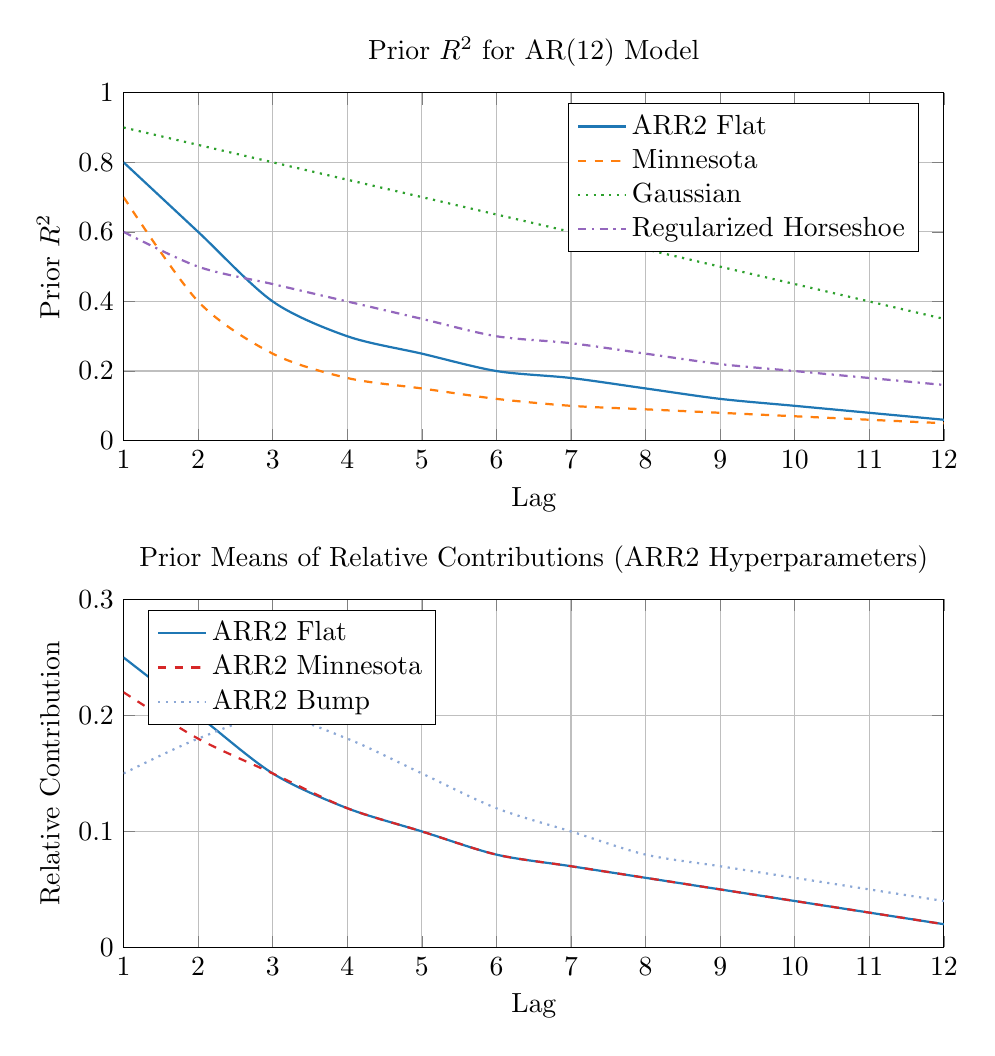
\begin{tikzpicture}
  % Top plot: Prior R^2 for AR(12)
  \begin{axis}[
    name=top_plot,
    height=6cm,
    width=12cm,
    xlabel={Lag},
    ylabel={Prior $R^2$},
    xmin=1, xmax=12,
    ymin=0, ymax=1,
    xtick={1,2,...,12},
    legend pos=north east,
    legend cell align={left},
    grid=both,
    title={Prior $R^2$ for AR(12) Model}
  ]
    % ARR2 Flat (blue)
    \addplot[smooth, arr2flatcolour, thick] coordinates {
      (1, 0.8) (2, 0.6) (3, 0.4) (4, 0.3) (5, 0.25) (6, 0.2) (7, 0.18) (8, 0.15) (9, 0.12) (10, 0.1) (11, 0.08) (12, 0.06)
    };
    
    % Minnesota (yellow)
    \addplot[smooth, minnesotacolour, thick, dashed] coordinates {
      (1, 0.7) (2, 0.4) (3, 0.25) (4, 0.18) (5, 0.15) (6, 0.12) (7, 0.1) (8, 0.09) (9, 0.08) (10, 0.07) (11, 0.06) (12, 0.05)
    };
    
    % Gaussian (green)
    \addplot[smooth, gaussiancolour, thick, dotted] coordinates {
      (1, 0.9) (2, 0.85) (3, 0.8) (4, 0.75) (5, 0.7) (6, 0.65) (7, 0.6) (8, 0.55) (9, 0.5) (10, 0.45) (11, 0.4) (12, 0.35)
    };
    
    % Regularized Horseshoe (purple)
    \addplot[smooth, rhscolour, thick, dashdotted] coordinates {
      (1, 0.6) (2, 0.5) (3, 0.45) (4, 0.4) (5, 0.35) (6, 0.3) (7, 0.28) (8, 0.25) (9, 0.22) (10, 0.2) (11, 0.18) (12, 0.16)
    };
    
    \legend{ARR2 Flat, Minnesota, Gaussian, Regularized Horseshoe}
  \end{axis}

  % Bottom plot: Prior means of relative contributions
  \begin{axis}[
    at=(top_plot.below south),
    anchor=north,
    yshift=-1cm,
    height=6cm,
    width=12cm,
    xlabel={Lag},
    ylabel={Relative Contribution},
    xmin=1, xmax=12,
    ymin=0, ymax=0.3,
    xtick={1,2,...,12},
    legend pos=north west,
    legend cell align={left},
    grid=both,
    title={Prior Means of Relative Contributions (ARR2 Hyperparameters)}
  ]
    % ARR2 Flat (blue)
    \addplot[smooth, arr2flatcolour, thick] coordinates {
      (1, 0.25) (2, 0.2) (3, 0.15) (4, 0.12) (5, 0.1) (6, 0.08) (7, 0.07) (8, 0.06) (9, 0.05) (10, 0.04) (11, 0.03) (12, 0.02)
    };
    
    % ARR2 Minnesota (red)
    \addplot[smooth, arr2minncolour, thick, dashed] coordinates {
      (1, 0.22) (2, 0.18) (3, 0.15) (4, 0.12) (5, 0.1) (6, 0.08) (7, 0.07) (8, 0.06) (9, 0.05) (10, 0.04) (11, 0.03) (12, 0.02)
    };
    
    % ARR2 Bump (light blue)
    \addplot[smooth, arr2bumpcolour, thick, dotted] coordinates {
      (1, 0.15) (2, 0.18) (3, 0.2) (4, 0.18) (5, 0.15) (6, 0.12) (7, 0.1) (8, 0.08) (9, 0.07) (10, 0.06) (11, 0.05) (12, 0.04)
    };
    
    \legend{ARR2 Flat, ARR2 Minnesota, ARR2 Bump}
  \end{axis}
\end{tikzpicture}
\end{document}